\section{Experimentos e resultados}\label{experimentos}
\subsection{Experimentos}
Para compreender o funcionamento do simulador NS-2 e tamb\'em estudar simula\c{c}\~oes de comunica\c{c}\~ao em cen\'arios militares, foram definidos dois experimentos te\'oricos, sendo o Experimento 1, um teste simples de converg\^encia de rotas, e o Experimento 2, baseado em estudos realizados por \cite{pereira}, o qual representa um caso de assalto e tomada de posi\c{c}\~ao inimiga.

Cada experimento possui suas caracter\'isticas, mas exite uma semelhan\c{c}a base, que \'e o tr\'afego que ir\'a caminhar pela rede, como comentado na se\c{c}\~ao \ref{trafegoDados}, o qual foi escolhido o CBR.

\subsubsection{Experimento 1}
O Experimento 1 baseia-se na ideia simples de um protocolo de rede \textit{ad hoc}, roteamento din\^amico.
O objetivo principal deste experimento \'e poder analisar o tempo de converg\^encia de roteamento de uma origem a um destino, alterando uma vez o caminho pelo qual eles realizam a comunica\c{c}\~ao.
A Tabela \ref{tabParamExp1} demonstra resumidamente os par\^ametros utilizados na execu\c{c}\~ao do Experimento 1.

\begin{table}[H]
	\centering
	\caption{Resumo dos par\^ametros usados no Experimento 1.}
	\begin{tabular}{ | l | l | }
		\hline
		N\'umero total de n\'os & 4 \\ \hline
		N\'umero de fontes de tr\'afego & 1 \\ \hline
		N\'umero de conex\~oes & 1 \\ \hline
		Tempo de simula\c{c}\~ao & 300 segundos \\ \hline
		\'Area total da simula\c{c}\~ao & 500x500 metros \\ \hline
		Tamanho dos pacotes & 512 \textit{bytes} \\ \hline	
		Velocidade dos n\'os & 1.5m/s constante \\ \hline
		Velocidade de banda & 11Mbps/s \\ \hline
	\end{tabular}
	\label{tabParamExp1}
\end{table}

A Figura \ref{figExp1} demonstra o experimento realizado, onde cada Soldado(n\'o) deve atingir seu respectivo Destino.
Cada Soldado inicia seu movimento a um tempo determinado na simula\c{c}\~ao, onde na Figura \ref{figExp1} \'e referenciado pelo prefixo \textit{at}, o qual \'e defido em segundos, e abaixo exibe o movimento de cada Soldado, onde nesse experimento todos os Soldados possuem um movimento constante de 1,5 metros por segundo. 

A fonte de tr\'afego nesse experimento \'e somente de uma, a qual realiza uma conex\~ao do Soldado 3(fonte) ao Soldado 1(destino). Inicialmente essa comunica\c{c}\~ao passar\'a pelo Soldado 2, pois os Soldados 1 e 3 n\~ao est\~ao pr\'oximos um do outro a fim de criarem uma rota direta.

\begin{figure}[H]
	\centering
	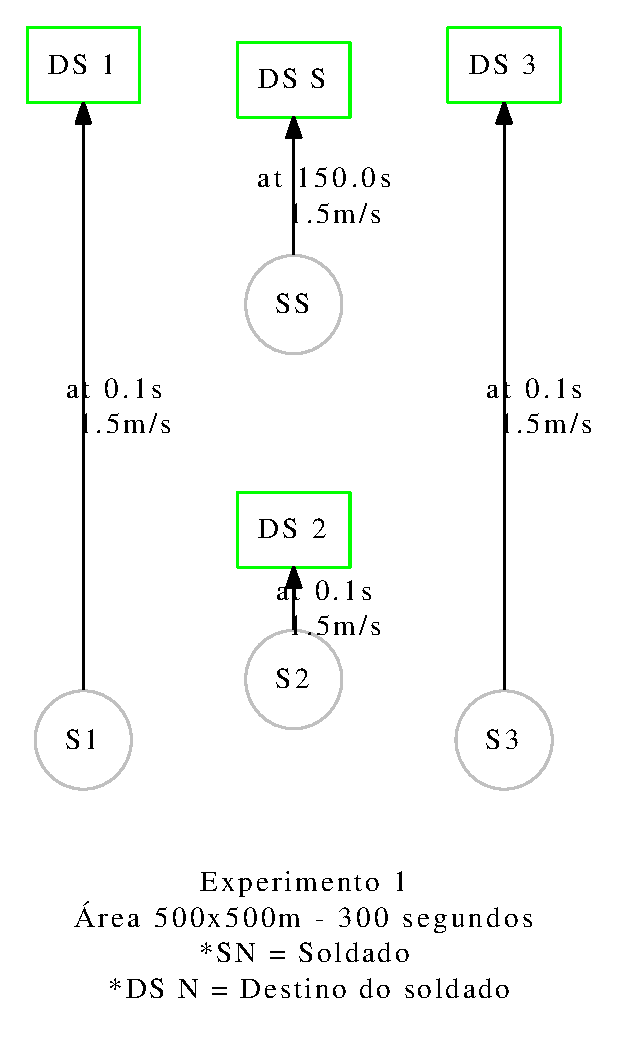
\includegraphics[scale=0.5]{experimento1.eps}
	\caption{Experimento 1}
	\label{figExp1}
\end{figure}

Observe que o Soldado 4 inicia somente seu movimento ao tempo de 150,0 segundos, enquanto os demais Soldados iniciam seus movimentos ao instante de 0,1 segundos.
Esses tempos de inicio de movimento foram definidos pelo fato do tempo em que o Soldado 2 precisa para atingir seu objetivo e parar de seguir em frente, enquanto os Soldados 1 e 3 continuam seus movimentos, e possam alcan\c{c}ar e estar dentro do raio de comunica\c{c}\~ao com o Soldado 4.
Quando os Soldados 1 e 3 se afastam do Soldado 2, eles perdem a sua rota por esse n\'o da rede, e necessitam buscar uma nova rota, a qual seguir\'a pelo Soldado 4, o qual nesse ponto poder\'a gerar dados diferentes de resultados.

\subsubsection{Experimento 2}
O Experimento 2 foi baseado em estudos realizados por \cite{pereira} em sua tese de mestrado. 
O objetivo deste experimento \'e analisar o desempenho dos protocolos de roteamento como um todo em um cen\'ario militar. 
\cite{pereira} comenta que esse \'e um cen\'ario t\'ipico de simula\c{c}\~ao de uma opera\c{c}\~ao de assalto e tomada de posi\c{c}\~ao inimiga.

Esse cen\'ario consiste em 4 grupos de soldados e 1 ve\'iculo de apoio, e cada grupo de soldados \'e formado por 4 soldados.
Cada grupo possui um comandante, o qual envia ordens aos outros soldados do grupo, e tamb\'em recebe e envia ordens do ve\'iculo de apoio, este qual \'e encarregado de repassar as ordens aos demais grupos.
Cada grupo nesse cen\'ario tem como objetivo tomar a posi\c{c}\~ao inimiga, onde na Figura \ref{figExp2} est\'a descrito como "Destino final".

\begin{figure}[H]
	\centering
	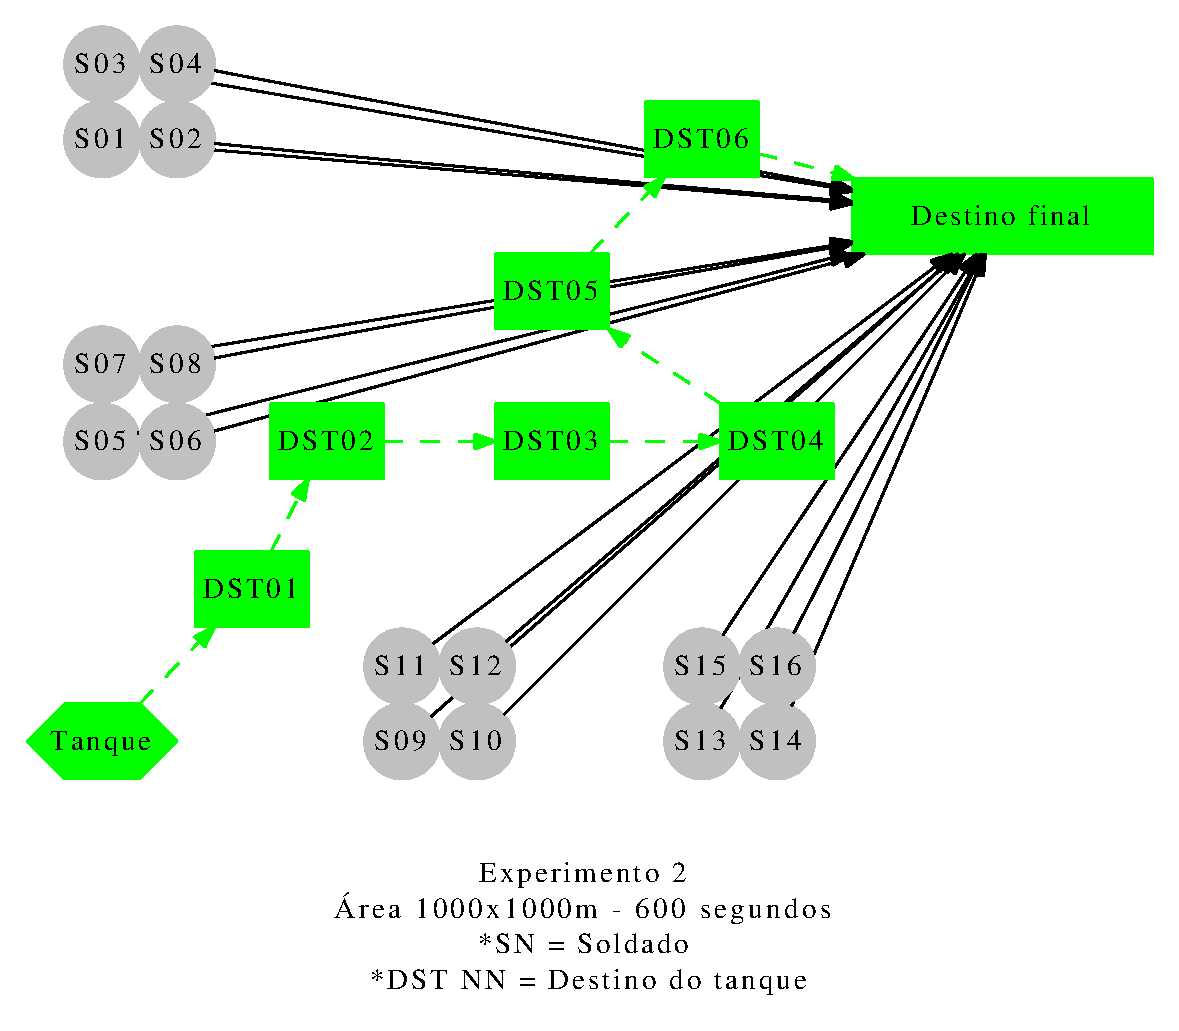
\includegraphics[scale=0.5]{experimento2.eps}
	\caption{Experimento 2}
	\label{figExp2}
\end{figure}

Todos os soldados de cada grupo dever\~ao avan\c{c}ar juntos durante o percurso do cen\'ario, n\~ao executando necessariamente um caminho em linha reta durante todo o trajeto.

A Tabela \ref{tabParamExp2} demonstra resumidamente os par\^ametros utilizados nesse experimento. 
Al\'em do tamanho, n\'umero de conex\~oes e n\'os diferentes do Experimento 1, podemos verificar que a velocidade dos n\'os possuem uma varia\c{c}\~ao.
Essa varia\c{c}\~ao ocorre pelo fato de que, os soldados recebem ordens de parada ou avan\c{c}o no percurso, sendo que em cada situa\c{c}\~ao \'e necess\'ario aumentar, diminuir ou at\'e mesmo parar o ritmo de avan\c{c}o no objetivo do cen\'ario.

\begin{table}[H]
	\centering
	\caption{Resumo dos par\^ametros usados no Experimento 2.}
	\begin{tabular}{ | l | l | }
		\hline
		N\'umero total de n\'os & 17 \\ \hline
		N\'umero de fontes de tr\'afego & 7 \\ \hline
		N\'umero de conex\~oes & 16 \\ \hline
		Tempo de simula\c{c}\~ao & 600 segundos \\ \hline
		\'Area total da simula\c{c}\~ao & 1000x1000 metros \\ \hline
		Tamanho dos pacotes & 512 \textit{bytes} \\ \hline
		Velocidade dos n\'os & 0 \`a 8 m/s constante \\ \hline
		Velocidade de banda & 11Mbps/s \\ \hline
	\end{tabular}
	\label{tabParamExp2}
\end{table}

\subsection{An\'alise comparativa dos resultados}

\subsubsection{Experimento 1}
Esta se\c{c}\~ao apresenta os resultados obtidos da simula\c{c}\~ao do Experimento 1.
Conforme os dados apresentados na Tabela \ref{tabExp1Result}, \'e poss\'ivel analisar que o protocolo AODV, o qual tem o modo de funcionamento reativo, possui uma taxa de entrega superior ao protocolo DSDV, que funciona em modo pr\'o-ativo, e ambos s\~ao baseados em Vetor de Dist\^ancias. 

A diferen\c{c}a na taxa de entrega ocorre pelo fato do AODV buscar uma rota para o destino no tempo em que \'e necess\'ario comunicar com esse mesmo destino, e o DSDV atualiza as rotas em intervalos distintos de tempo.
Quando a topologia muda no experimento, ou seja, a conex\~ao do Soldado 1 com o Soldado 3 altera o salto, pelo Soldado 2, para o Soldado 4, \'e necess\'ario que o protocolo altere a rota de comunica\c{c}\~ao dos Soldados.
Tal altera\c{c}\~ao vai depender como o protocolo funciona, e nesse caso, o modo reativo foi superior ao pr\'o-ativo com base em Vetor de Dist\^ancias.

Na execu\c{c}\~ao do experimento com o DSDV, considerando quando a comunica\c{c}\~ao ocorre pr\'oximo ao tempo de mudan\c{c}a da topologia da rede, o mesmo protocolo ainda n\~ao atualizou suas rotas, ent\~ao encaminha a comunica\c{c}\~ao por uma rota inv\'alida, e descarta os pacotes da comunica\c{c}\~ao. E o AODV, em tempo de execu\c{c}\~ao, consegue detectar a mudan\c{c}a da topologia.

\begin{table}[H]
	\centering
	\caption{Resultado das simula\c{c}\~oes do Experimento 1}
	\begin{tabular}{ | c | c | c | c | }
		\hline
		M\'ETRICAS AVALIADAS & DSDV & AODV & OLSR \\ \hline
		Taxa de entrega & 92.98\% & 99.83\% & 98.43\% \\ \hline
		Atraso m\'edio (ms) & 10.7575 & 11.4837 & 11.3047 \\ \hline
		N\'umero de pacotes & 543 & 588 & 565 \\ \hline
		N\'umero de \textit{bytes} & 288896 & 312816 & 300580 \\ \hline
	\end{tabular}
	\label{tabExp1Result}
\end{table}

Entretanto, quando um protocolo possui um funcionamento pr\'o-ativo, por\'em sendo baseado em Estado de Enlace, que \'e o caso do OLSR, percebe-se que a taxa de entrega aumenta em rela\c{c}\~ao ao DSVD, que \'e baseado em Vetor de Dist\^ancias.
Esse aumento ocorre porque, quando a topologia da rede do Experimento 1 \'e modificada, a base Estado de Enlace detecta a altera\c{c}\~ao de conex\~ao dos n\'os vizinhos, atualizando suas tabelas de rotas, o que altera o intervalo de atualiza\c{c}\~ao das rotas.

O objetivo inicial desse experimento era analisar o tempo de converg\^encia entre os protocolos, o qual n\~ao foi muito significativo.
Analisando os resultados de Atraso M\'edio de cada protocolo, percebe-se que as diferen\c{c}as foram menores de 1 ms entre os protocolos de roteamento, todos trabalhando pr\'oximos a 11 milissegundos.

Comparando as \'ultimas duas m\'etricas de desempenho, sendo elas, n\'umeros de pacotes e n\'umento de \textit{bytes}, pode-se analisar que o DSDV teve uma melhor efici\^encia quanto ao uso da rede. 
Esse resultado deve-se ao fato de que o AODV duplica os pacotes de roteamento, e \cite{ramachandran} comenta que o AODV n\~ao reutiliza informa\c{c}\~oes de roteamento, at\'e mesmo em casos comuns de comunica\c{c}\~ao.
J\'a o DSDV, mesmo atualizando as tabelas de roteamento a cada instante de tempo, pode reutilizar informa\c{c}\~oes, diminuindo o n\'umero de pacotes de roteamento. 

Os resultados do protocolo OLSR podem ser explicados pelo fato de que o mesmo atualiza suas rotas quando o Estado de Enlace muda. Assim, aumenta um pouco o n\'umero de pacotes em rela\c{c}\~ao ao DSDV, por\'em se demonstra eficiente com rela\c{c}\~ao ao AODV pela sua caracter\'istica pr\'o-ativa.

\subsubsection{Experimento 2}
Diferentemente do Experimento 1, o Experimento 2 possui caracter\'isticas espec\'ificas de mobilidade, em que cada soldado no cen\'ario n\~ao vai percorrer um caminho cont\'inuo, e tamb\'em, n\~ao vai ter uma velocidade constante de avan\c{c}o para o objetivo final do cen\'ario.
Foram gerados e executados 15 simula\c{c}\~oes de cen\'arios, e obtendo-se assim, um resultado de m\'edia somat\'oria entre os dados extra\'idos.
A Tabela \ref{tabExp2Result} demonstra a m\'edia destes resultados obtidos no Experimento 2.

Analisando a m\'etrica de Taxa de Entrega dos pacotes na simula\c{c}\~ao, pode-se observar que houve uma invers\~ao de desempenho entre o DSDV e o AODV, se comparado com o Experimento 1, pois o DSDV teve um resultado superior ao AODV.
Esse resultado pode ser explicado com base no tamanho total da rede, o qual teve um aumento significativo no n\'umero de n\'os que comp\~oem a simula\c{c}\~ao.
Como o modo de funcionamento do DSDV \'e pr\'o-ativo, ele mant\'em as tabelas de rotas para a comunica\c{c}\~ao. Em contrapartida, o AODV ter\'a que descobrir a rota antes de comunicar, por ser um protocolo reativo.
Como a rede desse experimento \'e maior, \'e poss\'ivel analisar que, dependendo do destino desejado, o AODV pode levar muito tempo para criar a comunica\c{c}\~ao, descartando os pacotes.

Essas mesmas caracter\'isticas, pr\'o-ativa e reativa, influenciam nos resultados da m\'etrica de desempenho de Atraso M\'edio, o qual o DSDV tem um resultado superior ao AODV, sendo mais r\'apido para entregar os pacotes.
A mesma caracter\'istica pr\'o-ativa pode explicar o resultado do protocolo OLSR tanto para as m\'etricas Taxa de Entrega como para o Atraso M\'edio.

\begin{table}[H]
	\centering
	\caption{Resultado das simula\c{c}\~oes do experimento 2}
	\begin{tabular}{ | c | c | c | c | }
		\hline
		M\'ETRICAS AVALIADAS & DSDV & AODV & OLSR \\ \hline
		Taxa de entrega & 96.88\% & 90.37\% & 95.29\%  \\ \hline
		Atraso m\'edio(ms) & 8.15969 & 16.3527 & 6.88545  \\ \hline
		N\'umero de pacotes & 7407 & 7696 & 7483  \\ \hline
		N\'umero de \textit{MegaBytes} & 3.76 & 3.90 & 3.80  \\ \hline
	\end{tabular}
	\label{tabExp2Result}
\end{table}

Analisando as m\'etricas N\'umero de Pacotes e N\'umero de \textit{MegaBytes}, percebe-se que o DSDV tamb\'em foi superior em rela\c{c}\~ao ao AODV na efici\^encia de roteamento.
Esse resultado foi favorecido pela caracter\'istica pr\'o-ativa em um experimento com um maior n\'umero de n\'os, logo que o DSDV n\~ao precisa buscar toda a topologia da rede toda a vez que necessita comunicar com o destino, que \'e o caso do AODV. 
O mesmo pode-se dizer do protocolo OLSR, por\'em, ele resultou em um n\'umero maior de pacotes que o DSDV por causa da sua base em Estado de Enlace, atualizando as tabelas de roteamento a cada mudan\c{c}a de conex\~ao dos n\'os vizinhos.


